\chapter{A new inverse model at 9800 rpm and PI tuning after DOB engagement}
\textit{Archived October study. All simulations, searches, and checks described below predate this report.}\par

\section{Scope and identification experiment}
Previous PILCO is replaced in this comparison by DOB98 + tuned PI. Base PI, retuned Poly2 + PID and smooth PILCO retain their earlier gains and traces. The new controller uses no quadratic feedforward. Its structure is PI minus a filtered input-disturbance estimate, followed by the common fuel limits.

A new nominal model is identified specifically at 9800 rpm (98\% rated speed), with zero external shaft load. After preparation, training applies a deterministic binary fuel perturbation of amplitude 0.035 lbm/s, switched approximately every 0.18 s for 30 s. The base PI stabilizes the experiment; identification uses actual applied fuel, including the excitation, and actual shaft speed. Independent validation uses the sum of 0.37 and 1.17 Hz sinusoids, with amplitudes 0.025 and 0.015 lbm/s. No validation samples enter the least-squares fit.

Let $y_k=N_k-9800$ and $v_k=u_k-u_0$, with $u_0=2.530351198$ lbm/s and $T_s=0.015$ s. A parsimonious local model is
\begin{equation}y_{k+1}=a y_k+b v_k,\qquad
a=0.9789097769,\quad b=9.3039586704.\end{equation}
The parameters minimize the squared one-step residual over the excited training interval. The identified pole is stable, and the numerator has no finite nonminimum-phase zero. The model is local: the training speed varies only a few rpm around 9800. Independent free-run fit is 99.7829\%, with 0.001406 rpm RMSE. Fit means $100(1-\|y-\hat y\|/\|y-\bar y\|)$.
\par\noindent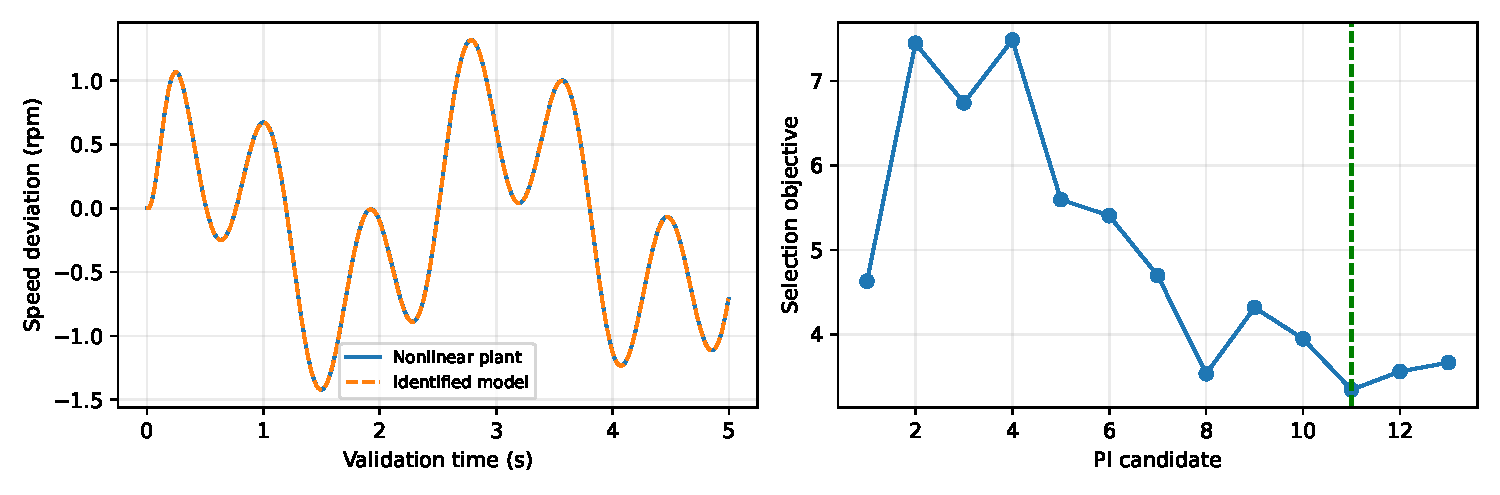
\includegraphics[width=\textwidth,height=.68\textheight,keepaspectratio]{late4_identification_tuning.pdf}
\section{Causal filtered inverse, step by step}
\textbf{1. Nominal speed dynamics.} With $q=z^{-1}$ denoting a one-sample delay,
\begin{equation}P_n(q)=\frac{bq}{1-aq}.\end{equation}
\textbf{2. Include the sensor.} Every controller retains the same physical sensor: time constant 0.05 s, unity gain, common initial conditions and noise disabled. The DOB uses its discrete approximation
\begin{equation}H_n(q)=\frac{(1-p)q}{1-pq},\qquad p=e^{-T_s/0.05}.\end{equation}
Thus the inverse is formed for sensed-speed dynamics $P_nH_n$. This approximation does not change the physical sensor blocks.

\textbf{3. Make the inverse causal and filtered.} Choose a unity-DC, two-pole low-pass filter with two delays:
\begin{equation}Q(q)=\frac{(1-r)^2q^2}{(1-rq)^2},\qquad r=e^{-2\pi f_cT_s},\quad f_c=1\ \mathrm{Hz}.\end{equation}
Then the two nominal delays cancel analytically:
\begin{equation}\frac{Q}{P_nH_n}=\frac{(1-r)^2(1-aq)(1-pq)}{b(1-p)(1-rq)^2}.\end{equation}
This is proper, causal and stable. A numerical frequency-response check verifies the identity, and an independent Python filter replay is compared with the recorded Simulink observer output.

\textbf{4. Estimate input-equivalent disturbance.} Use the known saturated command, without access to the external load signal:
\begin{equation}\hat d_{\rm raw}=\frac{Q}{P_nH_n}(N_s-N_0)-Q(u_{\rm cmd}-u_0).\end{equation}
The last estimate before absolute time 45 s is latched as a trim bias $d_0$. Compensation engages over the following two seconds, before the evaluation starts at 60 s:
\begin{equation}c=\operatorname{clip}\{0.7(\hat d_{\rm raw}-d_0),-1,1\},\qquad
u_{\rm cmd}=\operatorname{clip}\{u_{\rm PI}-c,0.2,4\}.\end{equation}
The compensation and fuel-command bounds are in lbm/s. The observer gain 0.7, cutoff 1 Hz and compensation limit 1 lbm/s are fixed engineering choices during the PI search; they are not claimed optimal.

\textbf{5. Tune PI after enabling the DOB.} The existing PI block uses $K_p(r-N_s)+K_i\int(r-N_s)dt$. Nine gain pairs, including the original (.025,.05), are followed by four local refinements. All candidates are evaluated with the DOB enabled on the requested combined cycle. Selection minimizes
\begin{equation}J=\mathrm{RMSE}_{0:25.005}+0.05R_{\rm seg},\end{equation}
where $R_{\rm seg}$ sums excess fuel total variation over 0--5, 5--10, 10--15 and 15--25.005 s. The weight is a numerical tuning weight with units rpm/(lbm/s). Invalid trajectories are rejected. This finite search selects $K_p=0.048$ and $K_i=0.05$; it does not establish a global optimum.
\section{Same combined cycle, revised four-controller comparison}
The target ramps from 9000 to 10000 rpm during relative seconds 0--5. A common 2789.650 hp external load is applied at second 10 and removed at second 15, followed by recovery through 25.005 s. The load is 10\% of the previously measured settled turbine power at 10000 rpm. Physical plant, sensor settings, reference, external load and fuel limits are matched. Saved comparator traces are reused because their implementations are unchanged.
\par\noindent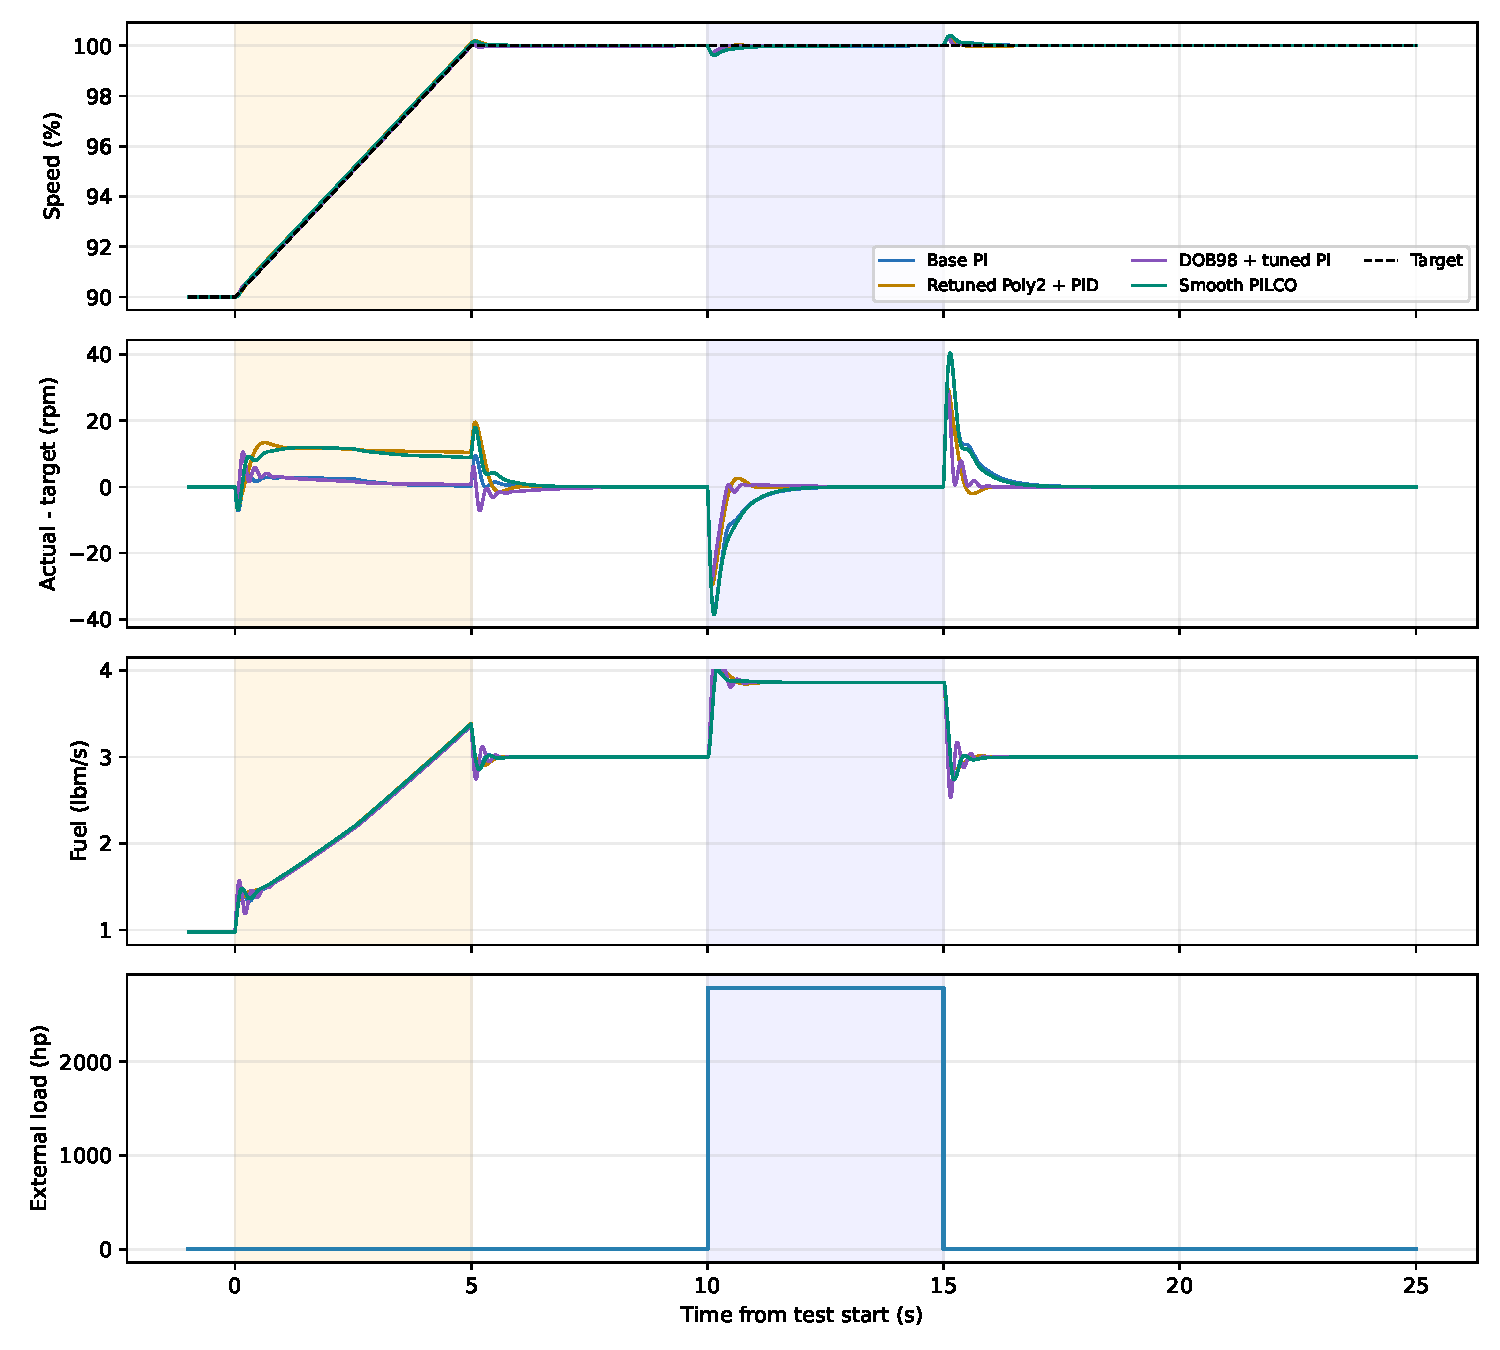
\includegraphics[width=\textwidth,height=.68\textheight,keepaspectratio]{late4_responses.pdf}
\section{Results and limits}
\begin{center}\small\begin{tabular}{lrrr}\toprule Controller & Ramp RMSE & Load/recovery RMSE & Full RMSE\\ & rpm & rpm & rpm\\\midrule
Base PI & 2.161 & 6.815 & 5.408 \\
Retuned Poly2 + PID & 10.949 & 4.416 & 6.214 \\
DOB98 + tuned PI & 2.459 & 3.710 & 3.142 \\
Smooth PILCO & 10.252 & 6.913 & 7.207 \\
\bottomrule\end{tabular}\end{center}
\begin{center}\small\begin{tabular}{lrrr}\toprule Controller & Load peak $|e|$ & Load excess TV & Min. surge\\ & rpm & lbm/s & \%\\\midrule
Base PI & 40.13 & 0.945 & 7.64 \\
Retuned Poly2 + PID & 29.39 & 0.696 & 7.75 \\
DOB98 + tuned PI & 29.10 & 2.184 & 7.74 \\
Smooth PILCO & 40.47 & 0.919 & 7.63 \\
\bottomrule\end{tabular}\end{center}
Errors use actual shaft speed, not sensed speed. Ramp RMSE covers 0--5 s; load/recovery RMSE covers 10--25.005 s; full RMSE covers the entire cycle. Load excess TV sums the 10--15 and 15--25.005 s segments. Sample interval is 0.015 s; first logged load-on is 10.005 s, and load-off is 15.000 s.

\textbf{Contribution of each change.} Base PI full-cycle RMSE is 5.408 rpm. Adding the DOB while retaining the original PI gains gives 4.546 rpm. Retuning PI with the DOB enabled gives 3.142 rpm. This ablation separates observer addition from gain tuning.

\textbf{Independent scenario check.} The selected gains are frozen and tested on a four-second speed ramp with a 5\% load pulse at seconds 10--15. Full-cycle RMSE is 2.024 rpm; minimum surge margin is 11.14\%. This check does not enter selection and is not a comparison against retuned baselines on that second scenario.

The requested combined cycle is a tuning case for DOB+PI, while the other gains were frozen from earlier studies. Consequently this is a comparison of the resulting controllers, not an equal-budget optimization contest. A local nominal model plus a DOB can tolerate some mismatch, but the small-excitation fit alone does not prove accuracy over 9000--10000 rpm. These nominal simulations are not a robust-stability proof. Fuel limits and compensation limits remain active parts of the implementation; the CSV records saturation and observer traces.
\section{Reproduction}
Run \path{dob98_identify_batch.m}, then \path{fit_dob98_model.py}, then \path{dob98_tune_batch.m}. The saved controller is \path{GasTurbine_DOB98_PI.mdl}, initialized by \path{tmats_dob98_setup.m}. Run \path{validate_dob98.py} for independent replay checks and \path{build_dob98_deliverables.py} for the revised figures and video. Data and selected parameters are under \path{results/dob98_pi_20261010}. Existing T-MATS workspace dependencies are required.
